\documentclass[11pt,a4paper]{article}

% ─── Core Packages ───────────────────────────────────────────────────────────
\usepackage[margin=0.9in]{geometry}
\usepackage[T1]{fontenc}
\usepackage{lmodern}
\usepackage{amsmath,amssymb,amsthm}
\usepackage{mathtools}
\usepackage{graphicx}
\usepackage{xcolor}
\usepackage{booktabs}
\usepackage{multirow}
\usepackage{array}
\usepackage{enumitem}
\usepackage{algorithm}
\usepackage{algpseudocode}
\usepackage{tcolorbox}
\usepackage{microtype}
\usepackage{caption}
\usepackage{subcaption}
\usepackage{tikz}
\usepackage{pgfplots}
\pgfplotsset{compat=1.18}
\usetikzlibrary{positioning,arrows.meta,shapes.geometric,fit,calc,decorations.pathreplacing}
\usepackage{listings}
\usepackage{tabularx}
\usepackage{longtable}
\usepackage{float}
\usepackage{fancyhdr}
\usepackage{titlesec}
\usepackage{hyperref}
\usepackage[noabbrev]{cleveref}

% ─── Page Style ──────────────────────────────────────────────────────────────
\pagestyle{fancy}
\fancyhf{}
\fancyhead[L]{\small\textsc{TC-ViTok: Complete Project Specification}}
\fancyhead[R]{\small\thepage}
\renewcommand{\headrulewidth}{0.4pt}

% ─── Color Definitions ───────────────────────────────────────────────────────
\definecolor{defbg}{RGB}{245,240,255}
\definecolor{defborder}{RGB}{130,70,200}
\definecolor{warnbg}{RGB}{255,245,235}
\definecolor{warnborder}{RGB}{200,130,70}
\definecolor{notebg}{RGB}{235,245,255}
\definecolor{noteborder}{RGB}{70,130,200}
\definecolor{implbg}{RGB}{235,255,240}
\definecolor{implborder}{RGB}{70,180,100}
\definecolor{keybg}{RGB}{255,250,230}
\definecolor{keyborder}{RGB}{200,170,50}
\definecolor{codegray}{RGB}{248,248,248}
\definecolor{codekey}{RGB}{0,0,180}
\definecolor{codecomment}{RGB}{100,100,100}
\definecolor{codestring}{RGB}{160,32,32}
\definecolor{phasecolor}{RGB}{40,80,160}

% ─── Listings Setup ──────────────────────────────────────────────────────────
\lstset{
  language=Python,
  basicstyle=\ttfamily\footnotesize,
  keywordstyle=\color{codekey}\bfseries,
  commentstyle=\color{codecomment}\itshape,
  stringstyle=\color{codestring},
  backgroundcolor=\color{codegray},
  frame=single, framerule=0.4pt, rulecolor=\color{gray!40},
  numbers=left, numberstyle=\tiny\color{gray}, numbersep=6pt,
  breaklines=true, showstringspaces=false, tabsize=2,
  xleftmargin=12pt, xrightmargin=4pt,
  aboveskip=8pt, belowskip=8pt,
}

% ─── tcolorbox Environments ──────────────────────────────────────────────────
\tcbuselibrary{skins,breakable}

\newtcolorbox{definitionbox}[1][]{
  enhanced, breakable,
  colback=defbg, colframe=defborder,
  fonttitle=\bfseries\small,
  left=6pt, right=6pt, top=4pt, bottom=4pt,
  arc=4pt, #1}

\newtcolorbox{warnbox}[1][]{
  enhanced, breakable,
  colback=warnbg, colframe=warnborder,
  fonttitle=\bfseries\small,
  left=6pt, right=6pt, top=4pt, bottom=4pt,
  arc=4pt, #1}

\newtcolorbox{notebox}[1][]{
  enhanced, breakable,
  colback=notebg, colframe=noteborder,
  fonttitle=\bfseries\small,
  left=6pt, right=6pt, top=4pt, bottom=4pt,
  arc=4pt, #1}

\newtcolorbox{implbox}[1][]{
  enhanced, breakable,
  colback=implbg, colframe=implborder,
  fonttitle=\bfseries\small,
  left=6pt, right=6pt, top=4pt, bottom=4pt,
  arc=4pt, #1}

\newtcolorbox{keybox}[1][]{
  enhanced, breakable,
  colback=keybg, colframe=keyborder,
  fonttitle=\bfseries\small,
  left=6pt, right=6pt, top=4pt, bottom=4pt,
  arc=4pt, #1}

\newtcolorbox{phasebox}[1][]{
  enhanced, breakable,
  colback=phasecolor!5, colframe=phasecolor,
  fonttitle=\bfseries,
  left=6pt, right=6pt, top=6pt, bottom=6pt,
  arc=4pt, #1}

% ─── Math Operators ──────────────────────────────────────────────────────────
\DeclareMathOperator*{\argmin}{arg\,min}
\DeclareMathOperator*{\argmax}{arg\,max}
\DeclareMathOperator{\Softmax}{Softmax}
\DeclareMathOperator{\TopK}{Top\text{-}k}
\DeclareMathOperator{\Concat}{Concat}
\DeclareMathOperator{\Upsample}{Upsample}
\DeclareMathOperator{\reshape}{reshape}
\DeclareMathOperator{\flatten}{flatten}
\DeclareMathOperator{\IoU}{IoU}
\DeclareMathOperator{\simop}{sim}
\DeclareMathOperator{\GELU}{GELU}
\newcommand{\sg}[1]{\mathrm{sg}\!\left[#1\right]}

% ─── Math Shorthands ─────────────────────────────────────────────────────────
\newcommand{\R}{\mathbb{R}}
\newcommand{\E}{\mathbb{E}}
\newcommand{\vc}{\mathbf{v}_c}
\newcommand{\qe}{\mathbf{q}_e}
\newcommand{\vm}{\mathbf{m}}
\newcommand{\vs}{\mathbf{s}}
\newcommand{\mI}{\mathbf{I}}
\newcommand{\mQ}{\mathbf{Q}}
\newcommand{\mV}{\mathbf{V}}

% ─── Theorem Environments ────────────────────────────────────────────────────
\newtheorem{hypothesis}{Hypothesis}
\newtheorem{remark}{Remark}
\newtheorem{definition}{Definition}
\newtheorem{proposition}{Proposition}

% ─── Section Formatting ─────────────────────────────────────────────────────
\titleformat{\section}
  {\Large\bfseries\color{phasecolor}}
  {\thesection}{1em}{}
\titleformat{\subsection}
  {\large\bfseries}
  {\thesubsection}{0.8em}{}

% ─── Hyperref Setup ──────────────────────────────────────────────────────────
\hypersetup{
  colorlinks=true,
  linkcolor=defborder,
  citecolor=teal,
  urlcolor=noteborder,
  pdftitle={TC-ViTok: Complete Project Specification},
  pdfauthor={Muhammad Ali Shah and Talha Hassan Ul Haq}
}

% ════════════════════════════════════════════════════════════════════════════
\begin{document}
% ════════════════════════════════════════════════════════════════════════════

\title{
  \textbf{TC-ViTok: Task-Conditioned Visual Tokenizer} \\[0.4em]
  \Large Complete Project Specification \\[0.3em]
  \large From Theory to Fully Buildable, Experimentally Validated System
}

\author{
  Muhammad Ali Shah - Talha Hassan Ul Haq \\[0.3em]
  Lahore University of Management Sciences (LUMS) \\
  \texttt{\{27100172, 27100306\}@lums.edu.pk}
}

\date{\today}

\maketitle
\thispagestyle{empty}

\begin{abstract}
This document provides a complete, end-to-end project specification for
\textbf{TC-ViTok} (Task-Conditioned Visual Tokenizer), a system that learns
to select visual tokens conditioned on the user's language query in
vision-language models. The specification spans deep theoretical
foundations, full mathematical derivations with tensor shapes at every step,
complete architecture design, step-by-step PyTorch implementation,
experimental validation strategy, failure mode catalog, and a week-by-week
execution roadmap. Every concept is bridged directly to implementation.
The document is structured so that a researcher or engineer can build,
train, evaluate, and publish the system directly from this specification.
\end{abstract}

\tableofcontents
\newpage

% ════════════════════════════════════════════════════════════════════════════
\section{Core Idea and System Overview}
\label{sec:overview}
% ════════════════════════════════════════════════════════════════════════════

\subsection{Problem Statement}

\begin{definitionbox}[title={The Fixed-Budget Problem}]
Vision-Language Models (VLMs) such as LLaVA-1.5 encode every input image
into a \textbf{fixed-length sequence} of $N = 576$ visual tokens (from a
$336 \times 336$ image with $14 \times 14$ patches). These tokens are
concatenated with $L$ text tokens and processed by a causal language model
(LLM). The self-attention cost in the LLM is:
\begin{equation}
  \text{Cost}_{\text{prefill}} = \mathcal{O}\bigl(N(N + L) + L^2\bigr).
  \label{eq:prefill_cost}
\end{equation}
For $N = 576$ and $L \approx 30$, visual tokens account for
$\sim\!95\%$ of prefill cost. \textbf{The core problem}: the visual token
budget is determined by image resolution, not by the task. A question
requiring localized reading (``What does the sign say?'') receives the
same 576 tokens as a question requiring only global understanding
(``Is this indoors?'').
\end{definitionbox}

\subsection{Why Current Methods Fail}

\begin{table}[h]
\centering
\caption{Limitations of existing visual token compression methods.}
\label{tab:existing_methods}
\renewcommand{\arraystretch}{1.2}
\small
\begin{tabular}{@{}lccll@{}}
  \toprule
  Method & Query-Aware & Where Saved & Core Limitation \\
  \midrule
  ToMe & No & ViT + LLM & Merges by visual similarity only \\
  LLaVA-PruMerge & No & LLM only & Uses {[CLS]} (whole-image summary) \\
  DynamicViT & No & ViT + LLM & Content-adaptive, task-agnostic \\
  BLIP-2 Q-Former & Partially & Both & Uses \emph{learned} queries, not user query \\
  \bottomrule
\end{tabular}
\end{table}

All existing methods share one limitation: \textbf{the compression decision
is made without knowledge of what the user is asking}.

\subsection{What TC-ViTok Does}

TC-ViTok introduces a \textbf{Tokenization Policy Network (TPN)}---a
lightweight cross-attention module that:
\begin{enumerate}[leftmargin=1.5em, itemsep=2pt]
  \item Takes the user's language query (encoded by frozen CLIP text
    encoder $\to \qe \in \R^{512}$).
  \item Takes a coarse spatial map of the image (from frozen DINOv2-S
    $\to \vc \in \R^{49 \times 384}$).
  \item Produces a binary mask
    $\vm \in \{0,1\}^{576}$ selecting exactly $k$ tokens.
  \item Applies this mask to the full ViT-L output before the LLM
    processes it.
\end{enumerate}

\textbf{The novelty}: the compression decision is conditioned on the
user's specific natural-language query.

\subsection{System Architecture}

\begin{figure}[t]
\centering
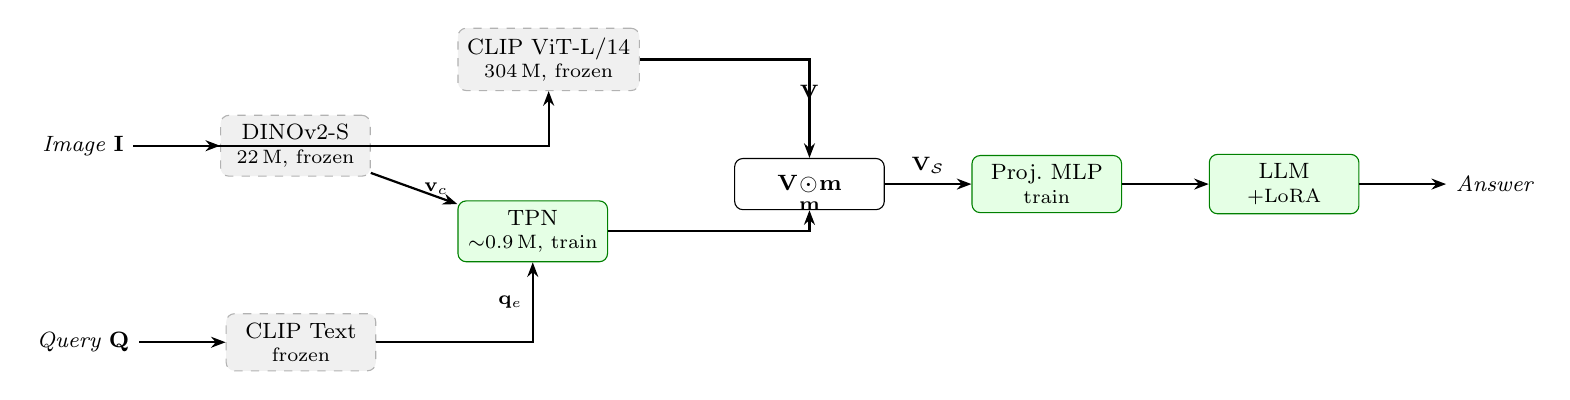
\begin{tikzpicture}[
    node distance=0.55cm and 1.1cm,
    block/.style={rectangle, draw, rounded corners=3pt,
                  minimum height=0.65cm, minimum width=1.9cm,
                  font=\footnotesize, align=center, fill=white},
    frozen/.style={block, fill=gray!12, draw=gray!60, dashed},
    trainable/.style={block, fill=green!10, draw=green!50!black},
    data/.style={font=\footnotesize\itshape, align=center},
    arr/.style={-{Stealth[scale=0.8]}, thick},
    label/.style={font=\scriptsize},
]
  % Input
  \node[data] (img) {Image $\mI$};
  \node[data, below=2.0cm of img] (query) {Query $\mQ$};
  % Encoders
  \node[frozen, right=of img] (dino)
    {DINOv2-S\\[-1pt]{\scriptsize 22\,M, frozen}};
  \node[frozen, right=of query] (clip)
    {CLIP Text\\[-1pt]{\scriptsize frozen}};
  \node[frozen, above right=0.3cm and 1.1cm of dino] (vit)
    {CLIP ViT-L/14\\[-1pt]{\scriptsize 304\,M, frozen}};
  % TPN
  \node[trainable, below right=0.3cm and 1.1cm of dino] (tpn)
    {TPN\\[-1pt]{\scriptsize $\sim$0.9\,M, train}};
  % Mask
  \node[block, right=1.6cm of tpn, yshift=0.6cm] (mask)
    {$\mV \!\odot\! \vm$};
  % Downstream
  \node[trainable, right=of mask] (mlp)
    {Proj.\ MLP\\[-1pt]{\scriptsize train}};
  \node[trainable, right=of mlp] (llm)
    {LLM\\[-1pt]{\scriptsize +LoRA}};
  \node[data, right=of llm] (ans) {Answer};
  % Arrows
  \draw[arr] (img) -- (dino);
  \draw[arr] (img) -| (vit);
  \draw[arr] (query) -- (clip);
  \draw[arr] (dino) -- (tpn)
    node[midway,right,label]{$\vc$};
  \draw[arr] (clip) -| (tpn)
    node[near end,left,label]{$\qe$};
  \draw[arr] (tpn) -| (mask)
    node[near end,above,label]{$\vm$};
  \draw[arr] (vit) -| (mask)
    node[near end,above,label]{$\mV$};
  \draw[arr] (mask) -- (mlp)
    node[midway,above,label]{$\mV_\mathcal{S}$};
  \draw[arr] (mlp) -- (llm);
  \draw[arr] (llm) -- (ans);
\end{tikzpicture}
\caption{TC-ViTok system architecture. Gray dashed: frozen components.
Green: trainable (TPN, projection MLP, LoRA adapters). The TPN produces a
binary mask $\vm$ conditioned on the query $\qe$ and coarse visual
features $\vc$, applied element-wise to the full ViT-L output $\mV$.}
\label{fig:architecture}
\end{figure}

\subsection{End-to-End Data Flow with Shapes}

\begin{table}[h]
\centering
\caption{Complete data flow through TC-ViTok with tensor shapes
(batch size $B$).}
\label{tab:data_flow}
\renewcommand{\arraystretch}{1.15}
\small
\begin{tabular}{@{}clllc@{}}
  \toprule
  Step & Operation & Input Shape & Output Shape & Frozen? \\
  \midrule
  1 & Resize for coarse & $(B,3,336,336)$ & $(B,3,98,98)$ & --- \\
  2 & DINOv2-S forward & $(B,3,98,98)$ & $(B,49,384)$ & Yes \\
  3 & CLIP text encode & Token IDs $(B,L)$ & $(B,512)$ & Yes \\
  4 & CLIP ViT-L/14 & $(B,3,336,336)$ & $(B,576,1024)$ & Yes \\
  5 & TPN: Q projection & $(B,512)$ & $(B,1,384)$ & No \\
  6 & TPN: K/V projection & $(B,49,384)$ & $(B,49,384)\times 2$ & No \\
  7 & TPN: cross-attn & Q,K,V & ctx$(B,384)$, $\alpha(B,49)$ & No \\
  8 & TPN: score MLP & $(B,433)$ & $(B,49)$ & No \\
  9 & TPN: upsample & $(B,1,7,7)$ & $(B,576)$ & No \\
  10 & Gumbel-STE/Top-$k$ & $(B,576)$ & $(B,576)$ binary & No \\
  11 & Mask application & $(B,576,1024)\!\odot\!(B,576,1)$ & $(B,576,1024)$ & --- \\
  12 & Projection MLP & $(B,576,1024)$ & $(B,576,4096)$ & No \\
  13 & Concat with text & Visual + Text & $(B,576{+}L,4096)$ & --- \\
  14 & LLM forward (+LoRA) & $(B,576{+}L,4096)$ & $(B,576{+}L,|\mathcal{V}|)$ & Partial \\
  \bottomrule
\end{tabular}
\end{table}

\subsection{Component Summary}

\begin{table}[h]
\centering
\caption{System components: parameters and trainability.}
\label{tab:components}
\renewcommand{\arraystretch}{1.15}
\small
\begin{tabular}{@{}lrcc@{}}
  \toprule
  Component & Parameters & Trainable & Role \\
  \midrule
  DINOv2-Small & 22\,M & No & Cheap spatial features for TPN \\
  CLIP Text Encoder & $\sim$63\,M & No & Query embedding \\
  CLIP ViT-L/14 & 304\,M & No & Full visual tokens \\
  \textbf{TPN} & \textbf{$\sim$0.9\,M} & \textbf{Yes}
    & \textbf{Query-conditioned spatial scoring} \\
  Projection MLP & $\sim$8\,M & Yes & Map visual $\to$ LLM space \\
  Vicuna-7B (LoRA) & 7\,B ($\sim$25\,M LoRA) & Partial
    & Answer generation \\
  \bottomrule
\end{tabular}
\end{table}

% ════════════════════════════════════════════════════════════════════════════
\section{Full Mathematical Foundation}
\label{sec:math}
% ════════════════════════════════════════════════════════════════════════════

\subsection{Complete Notation}

\begin{table}[t]
\centering
\caption{Complete notation reference.}
\label{tab:notation}
\renewcommand{\arraystretch}{1.2}
\small
\begin{tabular}{@{}llp{7cm}@{}}
  \toprule
  Symbol & Shape & Description \\
  \midrule
  \multicolumn{3}{@{}l}{\emph{Inputs}} \\
  $\mI$ & $H{\times}W{\times}3$ & Raw input image \\
  $\mI_c$ & $98{\times}98{\times}3$ & Image resized for coarse encoder \\
  $\mQ = (q_1,\ldots,q_L)$ & sequence & Language query tokens \\[3pt]
  \multicolumn{3}{@{}l}{\emph{Intermediate representations}} \\
  $\vc \in \R^{M \times d_c}$ & $49{\times}384$
    & Coarse DINOv2-S spatial features \\
  $\qe \in \R^{d_q}$ & $512$
    & CLIP text [EOS] embedding \\
  $\mV \in \R^{N \times d_v}$ & $576{\times}1024$
    & Full CLIP ViT-L/14 visual embeddings \\[3pt]
  \multicolumn{3}{@{}l}{\emph{TPN outputs}} \\
  $\vs_M \in \R^{M}$ & $49$
    & Coarse spatial relevance scores \\
  $\vs_N \in \R^{N}$ & $576$
    & Full-resolution scores (upsampled) \\
  $\vm \in \{0,1\}^{N}$ & $576$
    & Binary selection mask \\
  $\mathcal{S} \subseteq \{1,\ldots,N\}$ & $|\mathcal{S}|{=}k$
    & Selected token index set \\
  $\mV_{\mathcal{S}} \in \R^{N \times d_v}$ & $576{\times}1024$
    & Masked visual tokens \\[3pt]
  \multicolumn{3}{@{}l}{\emph{Hyperparameters}} \\
  $N = (H/p)^2$ & $576$ & Total visual tokens ($p{=}14$, $H{=}336$) \\
  $k$ & $144$ (default) & Token budget \\
  $\tau$ & scalar & Gumbel-Sigmoid temperature \\
  $\lambda, \mu, \nu$ & scalars & Loss coefficients \\
  \bottomrule
\end{tabular}
\end{table}

\subsection{The Optimization Objective}

\begin{definitionbox}[title={TC-ViTok Training Objective}]
\begin{equation}
  \theta^* = \argmin_{\theta} \;
    \E_{(\mI,\mQ,A)\sim\mathcal{D}} \Big[
      \underbrace{
        -\log P\!\left(A \mid \mQ,\,\mV_{\mathcal{S}_\theta}\right)
      }_{\mathcal{L}_{\text{VQA}}:\;\text{task fidelity}}
      \;+\; \underbrace{
        \lambda \cdot \frac{\lVert \vs_\theta \rVert_1}{N}
      }_{\mathcal{L}_{\text{comp}}:\;\text{sparsity}}
      \;+\; \underbrace{
        \mu \cdot \mathcal{L}_{\text{ent}}
      }_{\text{spatial diversity}}
    \Big]
  \label{eq:objective}
\end{equation}
where $\mathcal{S}_\theta = \TopK(\vs_\theta(\qe,\vc),\, k)$,
$A$ is the ground-truth answer, $\vs_\theta$ is the TPN score vector,
and $\mathcal{L}_{\text{ent}}$ is the spatial-entropy regularizer
(\cref{eq:entropy_reg}).
\end{definitionbox}

\paragraph{Variable-by-variable meaning.}
\begin{itemize}[leftmargin=1.5em, itemsep=1pt]
  \item $\theta$: All trainable parameters (TPN weights, LoRA matrices,
    MLP projector).
  \item $\mathcal{L}_{\text{VQA}}$: ``Can the LLM still answer correctly
    with only the selected tokens?'' Forces retention of task-relevant
    tokens.
  \item $\mathcal{L}_{\text{comp}}$: ``Are the raw scores sparse?''
    Differentiable proxy for sparsity (see below).
  \item $\mathcal{L}_{\text{ent}}$: ``Is the selection spatially diverse
    across a batch?'' Prevents center-bias collapse.
\end{itemize}

\paragraph{Why $\lVert\vs_\theta\rVert_1/N$ and not $|\mathcal{S}|/N$.}
Since $\mathcal{S}_\theta = \TopK(\vs_\theta, k)$ always returns exactly
$k$ indices:
\begin{equation}
  |\mathcal{S}_\theta| = k \;\; \forall\, \theta
  \qquad \Longrightarrow \qquad
  \frac{\partial}{\partial \theta}\!\left(\frac{|\mathcal{S}_\theta|}{N}\right)
  = \frac{\partial}{\partial \theta}\!\left(\frac{k}{N}\right) = 0.
\end{equation}
No gradient flows. Instead, $\|\vs_\theta\|_1 = \sum_{i=1}^{N} |s_i|$
\emph{is} differentiable because the scores $s_i$ are continuous TPN
outputs. Minimizing $\|\vs_\theta\|_1$ pushes most scores toward zero;
via the Gumbel-Sigmoid, near-zero scores map to near-zero selection
probabilities.

\paragraph{Policy class.}
\begin{equation}
  \pi_\theta(\qe,\vc) = \TopK\!\bigl(\vs_\theta(\qe,\vc),\; k\bigr),
  \label{eq:policy_class}
\end{equation}
which strictly subsumes query-agnostic methods: if query-conditioning
provides no signal, the TPN can learn to ignore $\qe$.

\subsection{Cross-Attention Derivation (Step-by-Step)}
\label{subsec:cross_attn_deriv}

\subsubsection{Input Setup}

\begin{itemize}[leftmargin=1.5em, itemsep=1pt]
  \item Query embedding: $\qe \in \R^{d_q}$, $d_q = 512$
  \item Coarse visual tokens: $\vc \in \R^{M \times d_c}$,
    $M = 49$, $d_c = 384$
  \item Model dimension: $d_{\text{model}} = 384$
  \item Heads: $H = 4$, per-head dimension: $d_k = 384/4 = 96$
\end{itemize}

\subsubsection{Step 1: Linear Projections}

\textbf{Query projection} (maps CLIP text space $\to$ shared space):
\begin{equation}
  \underbrace{\qe}_{1 \times 512}
  \cdot
  \underbrace{\mathbf{W}^Q}_{512 \times 384}
  \;=\;
  \underbrace{\mathbf{Q}_{\text{attn}}}_{1 \times 384}
  \label{eq:q_proj}
\end{equation}

\textbf{Key projection} (maps DINOv2 space $\to$ shared space):
\begin{equation}
  \underbrace{\vc}_{49 \times 384}
  \cdot
  \underbrace{\mathbf{W}^K}_{384 \times 384}
  \;=\;
  \underbrace{\mathbf{K}_{\text{attn}}}_{49 \times 384}
  \label{eq:k_proj}
\end{equation}

\textbf{Value projection}:
\begin{equation}
  \underbrace{\vc}_{49 \times 384}
  \cdot
  \underbrace{\mathbf{W}^V}_{384 \times 384}
  \;=\;
  \underbrace{\mathbf{V}_{\text{attn}}}_{49 \times 384}
  \label{eq:v_proj}
\end{equation}

\subsubsection{Step 2: Multi-Head Reshape}

Split each projection into $H = 4$ heads of dimension $d_k = 96$:
\begin{align}
  \mathbf{Q}_{\text{attn}} &\in \R^{1 \times 384}
    \xrightarrow{\text{reshape}} \R^{1 \times 4 \times 96}
    \xrightarrow{\text{transpose}} \R^{4 \times 1 \times 96} \\
  \mathbf{K}_{\text{attn}} &\in \R^{49 \times 384}
    \xrightarrow{\text{reshape}} \R^{49 \times 4 \times 96}
    \xrightarrow{\text{transpose}} \R^{4 \times 49 \times 96} \\
  \mathbf{V}_{\text{attn}} &\in \R^{49 \times 384}
    \xrightarrow{\text{reshape}} \R^{49 \times 4 \times 96}
    \xrightarrow{\text{transpose}} \R^{4 \times 49 \times 96}
\end{align}

With batch dimension $B$, shapes become:
$\mathbf{Q}\!: (B,4,1,96)$,\;
$\mathbf{K}\!: (B,4,49,96)$,\;
$\mathbf{V}\!: (B,4,49,96)$.

\subsubsection{Step 3: Scaled Dot-Product Attention}

For each head $h$:
\begin{equation}
  \text{logits}^{(h)} =
    \frac{\mathbf{Q}^{(h)} \cdot {\mathbf{K}^{(h)}}^\top}{\sqrt{d_k}}
\end{equation}
Shape derivation:
\begin{equation}
  \underbrace{\mathbf{Q}^{(h)}}_{B \times 1 \times 96}
  \cdot
  \underbrace{{\mathbf{K}^{(h)}}^\top}_{B \times 96 \times 49}
  \;=\;
  \underbrace{\text{logits}^{(h)}}_{B \times 1 \times 49}
\end{equation}
Division by $\sqrt{96} \approx 9.8$ prevents gradient saturation in the
softmax.

\textbf{Attention weights}:
\begin{equation}
  \boldsymbol{\alpha}^{(h)}
    = \Softmax(\text{logits}^{(h)})
    \in \R^{B \times 1 \times 49}
  \label{eq:attn_weights}
\end{equation}
Each $\alpha^{(h)}_j$ represents how strongly the query matches coarse
spatial position $j$ under head $h$. The distribution sums to 1 over the
49 positions.

\begin{notebox}[title={Intuition}]
If the query is ``What color is the car?'' and position $j{=}23$ contains
the car, then $\alpha^{(h)}_{23}$ should be large. The learned projections
$\mathbf{W}^Q$ and $\mathbf{W}^K$ align the CLIP text and DINOv2 visual
spaces so that semantic matching produces meaningful spatial attention.
\end{notebox}

\subsubsection{Step 4: Context Computation}

\begin{equation}
  \underbrace{\boldsymbol{\alpha}^{(h)}}_{B \times 1 \times 49}
  \cdot
  \underbrace{\mathbf{V}^{(h)}}_{B \times 49 \times 96}
  \;=\;
  \underbrace{\mathbf{a}^{(h)}}_{B \times 1 \times 96}
  \label{eq:context}
\end{equation}
This is a weighted average of value vectors, with weights proportional to
query-key similarity.

\subsubsection{Step 5: Multi-Head Concatenation and Output Projection}

\begin{equation}
  \underbrace{\Concat(\mathbf{a}^{(1)}, \ldots, \mathbf{a}^{(4)})}%
    _{B \times 1 \times 384}
  \cdot
  \underbrace{\mathbf{W}^O}_{384 \times 384}
  \;=\;
  \underbrace{\mathbf{a}}_{B \times 1 \times 384}
  \label{eq:multihead}
\end{equation}
After squeezing the singleton: $\mathbf{a} \in \R^{B \times 384}$.

\subsubsection{Step 6: Attention Weight Aggregation}

\begin{equation}
  \bar{\boldsymbol{\alpha}} =
    \frac{1}{H}\sum_{h=1}^{H} \boldsymbol{\alpha}^{(h)}
    \in \R^{B \times 1 \times 49}
    \;\xrightarrow{\text{squeeze}}\;
    \R^{B \times 49}
  \label{eq:alpha_avg}
\end{equation}

\begin{remark}
  The context vector $\mathbf{a}$ is a single $d_{\text{model}}$-dimensional
  vector that has lost explicit spatial structure. The attention weights
  $\bar{\boldsymbol{\alpha}}$ directly encode ``which spatial position was
  attended to,'' preserving spatial information that the score MLP needs.
  This concatenation forms a \emph{residual spatial connection}.
\end{remark}

\subsection{Spatial Scoring Derivation}
\label{subsec:score_deriv}

\subsubsection{Score MLP}

Input: concatenation of context and averaged attention weights:
\begin{equation}
  \mathbf{x} = [\mathbf{a}^{\flat};\;
    \bar{\boldsymbol{\alpha}}^{\flat}]
    \in \R^{B \times (384 + 49)}
    = \R^{B \times 433}
\end{equation}
where $\mathbf{x}^{\flat}$ denotes squeezing the singleton dimension.

Hidden layer:
\begin{equation}
  \mathbf{h} = \GELU(\mathbf{W}_1 \mathbf{x} + \mathbf{b}_1)
    \in \R^{B \times d_h}
  \label{eq:score_hidden}
\end{equation}
with $\mathbf{W}_1 \in \R^{d_h \times 433}$, $d_h = 512$.

Output layer:
\begin{equation}
  \vs_M = \mathbf{W}_2 \mathbf{h} + \mathbf{b}_2
    \in \R^{B \times 49}
  \label{eq:score_output}
\end{equation}
with $\mathbf{W}_2 \in \R^{49 \times 512}$. Each element $s_{M,j}$ is a
scalar relevance score for coarse spatial position $j$.

\subsubsection{Bilinear Upsampling}

The 49 coarse scores map to 576 fine-grained scores:
\begin{equation}
  \vs_M \in \R^{B \times 49}
  \xrightarrow{\text{reshape}} \R^{B \times 1 \times 7 \times 7}
  \xrightarrow{\text{bilinear}} \R^{B \times 1 \times 24 \times 24}
  \xrightarrow{\text{flatten}} \R^{B \times 576}
  = \vs_N
  \label{eq:upsample}
\end{equation}

\textbf{Coordinate mapping.} For target position $(x', y')$ in the
$24 \times 24$ grid, the source position in the $7 \times 7$ grid is:
\begin{equation}
  x = x' \cdot \frac{7-1}{24-1} = x' \cdot \frac{6}{23},
  \qquad
  y = y' \cdot \frac{6}{23}
\end{equation}

\textbf{Interpolation formula.} For non-integer source coordinate $(x,y)$:
\begin{equation}
  s_N(x',y') = \sum_{i \in \{0,1\}} \sum_{j \in \{0,1\}}
    s_M(\lfloor x \rfloor{+}i,\, \lfloor y \rfloor{+}j)
    \cdot (1 - |x - \lfloor x \rfloor - i|)
    \cdot (1 - |y - \lfloor y \rfloor - j|)
\end{equation}
This is differentiable w.r.t.\ the source values $s_M$, so gradients
flow through the upsampling layer.

\paragraph{Inductive bias.}
Bilinear upsampling enforces \emph{spatial contiguity}: if a
$7 \times 7$ region is relevant, all $\sim\!3.4 \times 3.4$ corresponding
patches in the $24 \times 24$ grid receive elevated scores. Relevant
image regions (faces, text blocks, signs) typically span multiple patches,
making this a sensible prior.

\subsection{Gumbel-Sigmoid Derivation}
\label{subsec:gumbel_deriv}

\subsubsection{The Non-Differentiability Problem}

The top-$k$ mask is a step function with zero derivative almost everywhere:
\begin{equation}
  m_i = \begin{cases}
    1 & \text{if } s_{N,i} \geq s_{N,(k)} \\
    0 & \text{otherwise}
  \end{cases}
  \qquad \Longrightarrow \qquad
  \frac{\partial m_i}{\partial s_{N,i}} =
    \delta(s_{N,i} - s_{N,(k)}) \approx 0 \text{ (a.e.)}
\end{equation}

\subsubsection{Why Not Gumbel-Softmax?}

Gumbel-Softmax produces a categorical distribution:
$\tilde{p}_i = \exp((s_i + g_i)/\tau) / \sum_j \exp((s_j + g_j)/\tau)$,
satisfying $\sum_i \tilde{p}_i = 1$ (``select exactly one token''). This
is inappropriate for top-$k$ where we need $k$ tokens simultaneously.

\subsubsection{Gumbel-Sigmoid: Independent Binary Decisions}

\begin{definitionbox}[title={Gumbel-Sigmoid Soft Mask}]
\textbf{Step 1}: Sample Gumbel$(0,1)$ noise.
For $u_i \sim \text{Uniform}(0,1)$, clamped to
$u_i \in [\epsilon, 1{-}\epsilon]$ with $\epsilon = 10^{-8}$:
\begin{equation}
  g_i = -\log(-\log(u_i))
\end{equation}

\textbf{Step 2}: Apply sigmoid with temperature:
\begin{equation}
  \tilde{m}_i(\tau) = \sigma\!\left(\frac{s_{N,i} + g_i}{\tau}\right)
    = \frac{1}{1 + \exp\!\left(-\frac{s_{N,i} + g_i}{\tau}\right)}
  \label{eq:gumbel_sigmoid}
\end{equation}
Each $\tilde{m}_i \in (0,1)$ independently. $\sum_i \tilde{m}_i$ is
\textbf{not} constrained to equal $k$.
\end{definitionbox}

\textbf{Key properties:}
\begin{itemize}[leftmargin=1.5em, itemsep=1pt]
  \item $\tau \to 0$:
    $\tilde{m}_i \to \mathbf{1}[s_{N,i} + g_i > 0]$ (binary).
  \item $\tau \to \infty$:
    $\tilde{m}_i \to 0.5$ (uniform, maximum-entropy gradient).
\end{itemize}

\textbf{Gradient computation:}
\begin{equation}
  \frac{\partial \tilde{m}_i}{\partial s_{N,i}}
    = \frac{1}{\tau} \cdot \tilde{m}_i(1 - \tilde{m}_i)
  \label{eq:gumbel_grad}
\end{equation}

\begin{table}[h]
\centering
\caption{Gradient magnitude as a function of temperature and mask value.}
\label{tab:grad_magnitude}
\renewcommand{\arraystretch}{1.15}
\small
\begin{tabular}{@{}cccl@{}}
  \toprule
  $\tau$ & Typical $\tilde{m}_i$ &
    $\frac{1}{\tau}\tilde{m}_i(1{-}\tilde{m}_i)$ & Behavior \\
  \midrule
  1.0 & $\sim$0.5 & $\sim$0.25 & All tokens get gradient \\
  0.55 & $\sim$0.3 or 0.7 & $\sim$0.38 & Selected tokens get more \\
  0.1 & $\sim$0.01 or 0.99 & $\sim$0.1 & Only boundary tokens \\
  \bottomrule
\end{tabular}
\end{table}

\subsubsection{STE Construction}

\begin{definitionbox}[title={Straight-Through Estimator for Top-$k$}]
\begin{align}
  \vm_{\text{hard}} &= \mathbf{1}[\vs_N \geq \tau_k(\vs_N)]
    && \text{(hard top-}k\text{ mask, forward pass)}
    \label{eq:hard} \\[3pt]
  \tilde{\vm}(\tau) &= \sigma((\vs_N + \mathbf{g})/\tau)
    && \text{(Gumbel-Sigmoid, backward pass)}
    \label{eq:soft} \\[3pt]
  \vm_{\text{STE}} &= \vm_{\text{hard}} - \sg{\tilde{\vm}(\tau)}
    + \tilde{\vm}(\tau)
    \label{eq:ste}
\end{align}
where $\tau_k(\vs_N)$ is the $k$-th largest value and $\sg{\cdot}$ is the
stop-gradient operator.
\end{definitionbox}

\textbf{Proof that this works:}

\emph{Forward pass:}
\begin{equation}
  \vm_{\text{STE}} = \vm_{\text{hard}} - \tilde{\vm} + \tilde{\vm}
    = \vm_{\text{hard}} \quad \checkmark
\end{equation}

\emph{Backward pass:}
\begin{equation}
  \frac{\partial \vm_{\text{STE}}}{\partial \vs_N}
    = \underbrace{
      \frac{\partial \vm_{\text{hard}}}{\partial \vs_N}
    }_{=\,0}
    - \underbrace{
      \frac{\partial \sg{\tilde{\vm}}}{\partial \vs_N}
    }_{=\,0}
    + \frac{\partial \tilde{\vm}}{\partial \vs_N}
    = \frac{\partial \tilde{\vm}}{\partial \vs_N}
    \quad \checkmark
\end{equation}

\subsection{Temperature Annealing}

\begin{equation}
  \tau(t) = \tau_{\max} - (\tau_{\max} - \tau_{\min}) \cdot \frac{t}{T}
  \label{eq:tau_schedule}
\end{equation}
with $\tau_{\max} = 1.0$, $\tau_{\min} = 0.1$, $T$ = total training steps.

\begin{notebox}[title={Why anneal?}]
At high $\tau$, the gradient $\tilde{m}_i(1{-}\tilde{m}_i)/\tau \approx 0.25$
is large for \emph{every} token---rich, low-variance learning signal.
As $\tau$ decreases, gradient concentrates on boundary tokens. Late
training thus resembles hard inference-time decisions.
\end{notebox}

\subsection{Compression Regularization Schedule}

\begin{equation}
  \lambda(t) = \lambda_{\max} \cdot
    \min\!\left(1,\; \frac{t}{T_{\text{warmup}}}\right)
  \label{eq:lambda_schedule}
\end{equation}
Early training ($\lambda \approx 0$): TPN learns \emph{what} to select.
Late training ($\lambda = \lambda_{\max}$): TPN learns to select
\emph{sparsely}.

\subsection{Entropy Regularizer}

\textbf{Goal}: prevent the TPN from always selecting the same positions.

Batch selection frequency for position $i$:
\begin{equation}
  \bar{m}_i = \frac{1}{B}\sum_{b=1}^{B} m_i^{(b)},
  \qquad
  \hat{p}_i = \frac{\bar{m}_i}{\sum_{j=1}^{N} \bar{m}_j + \epsilon}
\end{equation}

Shannon entropy:
\begin{equation}
  \mathcal{L}_{\text{ent}}
    = -\sum_{i=1}^{N} \hat{p}_i \log(\hat{p}_i + \epsilon)
  \label{eq:entropy_reg}
\end{equation}

Maximum entropy: $\mathcal{L}_{\text{ent}}^{\max} = \log N = \log 576
\approx 6.36$ (uniform selection). Minimum: $\mathcal{L}_{\text{ent}}
\to 0$ (fixed selection). We \emph{maximize} entropy by setting $\mu < 0$
(equivalently, subtracting $|\mu| \cdot \mathcal{L}_{\text{ent}}$).

\subsection{Query-Diversity Loss}

For two queries $\qe_1^{(b)}, \qe_2^{(b)}$ on image $b$:
\begin{equation}
  \mathcal{L}_{\text{div}} = \sum_{b=1}^{B}
    \max\!\bigl(0,\;
      \simop(\vm_1^{(b)}, \vm_2^{(b)}) - \gamma
    \bigr)
    \cdot
    \bigl(1 - \simop(\qe_1^{(b)}, \qe_2^{(b)})\bigr)
  \label{eq:div_loss}
\end{equation}
where $\simop(\mathbf{a},\mathbf{b}) = \mathbf{a}^\top\mathbf{b} /
(\|\mathbf{a}\|\|\mathbf{b}\|)$ and $\gamma$ is a margin ($\gamma = 0.5$).

\subsection{Complete Unified Loss}

\begin{definitionbox}[title={Full Training Loss}]
\begin{equation}
  \mathcal{L}(t) =
    \underbrace{-\log P(A \mid \mQ, \mV_{\mathcal{S}})}_{\text{VQA}}
    + \underbrace{\lambda(t) \cdot \frac{\|\vs_N\|_1}{N}}_{\text{sparsity}}
    - \underbrace{|\mu| \cdot \mathcal{L}_{\text{ent}}}_{\text{diversity}}
    + \underbrace{\nu \cdot \mathcal{L}_{\text{div}}}_{\text{query diversity}}
  \label{eq:total_loss}
\end{equation}
Default coefficients: $\lambda_{\max} = 0.1$, $|\mu| = 0.01$,
$\nu = 0.01$, $\gamma = 0.5$.
\end{definitionbox}

% ════════════════════════════════════════════════════════════════════════════
\section{Architecture Deep Dive}
\label{sec:architecture}
% ════════════════════════════════════════════════════════════════════════════

\subsection{Component 1: Coarse Visual Encoder (DINOv2-Small)}

\paragraph{What it does.}
Produces a low-resolution spatial feature map. Each of the 49 output tokens
corresponds to a $14 \times 14$ pixel region of the $98 \times 98$ input.

\paragraph{Why it exists.}
The TPN needs ``what is where'' information. Using the full ViT-L would
cost as much as the computation we save. DINOv2-S is $14\times$ smaller
and runs at $6\times$ lower resolution.

\paragraph{Specification.}
\begin{itemize}[leftmargin=1.5em, itemsep=1pt]
  \item Architecture: ViT-Small (12 layers, 6 heads, 384 hidden dim)
  \item Patch size: 14, input: $98 \times 98 \Rightarrow 7 \times 7 = 49$
    spatial tokens
  \item Input: $(B, 3, 98, 98)$ with ImageNet normalization
  \item Output: $(B, 49, 384)$ (CLS token excluded)
  \item Parameters: 22\,M (all frozen)
\end{itemize}

\paragraph{Why DINOv2, not CLIP?}
DINOv2's self-supervised local-feature objective produces spatial tokens
that faithfully correspond to image regions. CLIP collapses spatial
structure into a global embedding; its spatial tokens are less
geometrically interpretable.

\begin{warnbox}[title={Critical Normalization Warning}]
DINOv2 uses ImageNet normalization:
\texttt{mean=[0.485, 0.456, 0.406]}, \texttt{std=[0.229, 0.224, 0.225]}.
CLIP uses different statistics:
\texttt{mean=[0.481, 0.458, 0.408]}, \texttt{std=[0.269, 0.261, 0.276]}.
Applying CLIP normalization to DINOv2 is a \textbf{silent, hard-to-debug
error} that degrades performance without raising exceptions.
\end{warnbox}

\subsection{Component 2: Text Encoder (CLIP ViT-B/32)}

\paragraph{Specification.}
\begin{itemize}[leftmargin=1.5em, itemsep=1pt]
  \item Architecture: 12-layer transformer, 8 heads, 512 hidden dim
  \item Input: tokenized query $(B, L_{\max})$, $L_{\max} = 77$ for CLIP
  \item Output: $\qe \in \R^{B \times 512}$ (the [EOS] token embedding)
  \item All frozen during training
\end{itemize}

\paragraph{Why [EOS] over mean-pooling?}
CLIP's contrastive training objective concentrates global query semantics
in the [EOS] position. Mean-pooling dilutes this with padding tokens that
were not optimized for this purpose.

\subsection{Component 3: Tokenization Policy Network (TPN)}

\paragraph{What it does.}
Maps $(\qe, \vc) \mapsto \vs_N \in \R^N$, producing a relevance score
for each of the $N$ full-resolution visual tokens.

\paragraph{Why it exists.}
This is the \textbf{novel component}. It operationalizes the thesis that
token selection should be conditioned on the user's question.

\paragraph{Internal pipeline.}
\begin{enumerate}[leftmargin=1.5em, itemsep=1pt]
  \item \textbf{Query projection}:
    $\qe\,(B,512) \xrightarrow{\mathbf{W}^Q} (B,1,384)$
  \item \textbf{Key/Value projection}:
    $\vc\,(B,49,384) \xrightarrow{\mathbf{W}^K, \mathbf{W}^V}
    (B,49,384)$ each
  \item \textbf{Multi-head cross-attention}:
    $\to$ context $(B,384)$, weights $(B,49)$
  \item \textbf{Score MLP}:
    $[\text{ctx};\alpha_{\text{avg}}]\,(B,433) \to (B,49)$
  \item \textbf{Bilinear upsample}:
    $(B,1,7,7) \to (B,1,24,24) \to (B,576)$
  \item \textbf{Mask generation}: Gumbel-STE (train) or Top-$k$ (infer)
\end{enumerate}

\paragraph{Parameter count.}

\begin{table}[h]
\centering
\caption{TPN parameter count with $d_q{=}512$, $d_c{=}d_{\text{model}}{=}384$,
$H{=}4$, $d_h{=}512$, $M{=}49$.}
\label{tab:tpn_params}
\renewcommand{\arraystretch}{1.15}
\small
\begin{tabular}{@{}lr@{}}
  \toprule
  Component & Parameters \\
  \midrule
  $\mathbf{W}^Q$ ($512 \times 384$) & 196{,}608 \\
  $\mathbf{W}^K$ ($384 \times 384$) & 147{,}456 \\
  $\mathbf{W}^V$ ($384 \times 384$) & 147{,}456 \\
  $\mathbf{W}^O$ ($384 \times 384$) & 147{,}456 \\
  LayerNorm $\times$ 2 & 1{,}634 \\
  Score MLP $\mathbf{W}_1$ ($433 \times 512$ + bias) & 222{,}208 \\
  Score MLP $\mathbf{W}_2$ ($512 \times 49$ + bias) & 25{,}137 \\
  \midrule
  \textbf{Total} & \textbf{887{,}955 ($\approx$0.9\,M)} \\
  \bottomrule
\end{tabular}
\end{table}

\begin{remark}
With two stacked cross-attention layers and $d_h = 1024$, the count
reaches $\approx$2.4\,M. The exact configuration should be reported.
\end{remark}

\subsection{Component 4: Mask Application}

Given $\vm \in \{0,1\}^N$ and $\mV \in \R^{N \times d_v}$:
\begin{equation}
  (\mV_{\mathcal{S}})_i = m_i \cdot \mV_i,
    \qquad i = 1, \ldots, N
  \label{eq:masking}
\end{equation}

\textbf{Option A --- Zero masking} (simpler):
\begin{equation}
  \mV_{\mathcal{S}} = \mV \odot \vm^{\uparrow}
  \qquad \text{where } \vm^{\uparrow} = \vm.\text{unsqueeze}(-1)
    \in \R^{B \times N \times 1}
\end{equation}
Retains length $N$; saves KV-cache memory but not FLOPs.

\textbf{Option B --- Gather} (efficient):
extract only selected tokens, producing sequence of length $k$.
Saves both FLOPs and memory. Requires variable-length batch handling.

\paragraph{Computational overhead of TPN pipeline.}
\begin{itemize}[leftmargin=1.5em, itemsep=1pt]
  \item DINOv2-S forward: $\sim$3\,ms on A100
  \item CLIP text encoding: $\sim$2\,ms
  \item TPN forward: $\sim$0.5\,ms
  \item \textbf{Total overhead}: $\sim$5.5\,ms
  \item \textbf{LLM savings} (576 $\to$ 144 tokens): $\sim$40\,ms
  \item \textbf{Net savings}: $\sim$34\,ms per sample
\end{itemize}

% ════════════════════════════════════════════════════════════════════════════
\section{Full Implementation Guide}
\label{sec:implementation}
% ════════════════════════════════════════════════════════════════════════════

\subsection{Stage A: Environment Setup}

\begin{implbox}[title={Required Libraries}]
\begin{lstlisting}[numbers=none, language=bash]
# Core ML
pip install torch==2.1.0 torchvision==0.16.0
pip install transformers==4.36.2 accelerate==0.25.0 peft==0.7.1

# Vision encoders
pip install timm==0.9.12

# Data and evaluation
pip install datasets==2.16.0 h5py==3.10.0 Pillow==10.1.0
pip install pycocoevalcap

# Logging
pip install wandb tqdm
\end{lstlisting}
\end{implbox}

\begin{table}[h]
\centering
\caption{Required model checkpoints.}
\label{tab:checkpoints}
\renewcommand{\arraystretch}{1.15}
\small
\begin{tabular}{@{}llr@{}}
  \toprule
  Model & HuggingFace ID & Size \\
  \midrule
  LLaVA-1.5-7B & \texttt{llava-hf/llava-1.5-7b-hf} & $\sim$13.5\,GB \\
  DINOv2-Small & \texttt{facebook/dinov2-small} & $\sim$88\,MB \\
  CLIP ViT-B/32 & \texttt{openai/clip-vit-base-patch32} & $\sim$340\,MB \\
  \bottomrule
\end{tabular}
\end{table}

\begin{table}[h]
\centering
\caption{Hardware requirements.}
\label{tab:hardware}
\renewcommand{\arraystretch}{1.15}
\small
\begin{tabular}{@{}lcccl@{}}
  \toprule
  Config & GPU & VRAM & Batch & Notes \\
  \midrule
  Minimum & 1$\times$ A100-40GB & 40\,GB & 1
    & Gradient checkpointing required \\
  Recommended & 1$\times$ A100-80GB & 80\,GB & 2--4
    & Comfortable margin \\
  Fast & 4$\times$ A100-80GB & 320\,GB & 16
    & Data-parallel training \\
  \bottomrule
\end{tabular}
\end{table}

\subsection{Stage B: Data Pipeline}

\subsubsection{Image Preprocessing}

\begin{lstlisting}[caption={Separate preprocessing for DINOv2 and CLIP.}]
from torchvision import transforms

# DINOv2 preprocessing (ImageNet normalization)
dino_transform = transforms.Compose([
    transforms.Resize((98, 98)),
    transforms.ToTensor(),
    transforms.Normalize(
        mean=[0.485, 0.456, 0.406],
        std=[0.229, 0.224, 0.225]
    )
])

# CLIP ViT-L preprocessing (handled by LLaVA processor):
# Resize to 336x336, CLIP normalization:
# mean=[0.48145466, 0.4578275, 0.40821073]
# std=[0.26862954, 0.26130258, 0.27577711]
\end{lstlisting}

\subsubsection{Feature Pre-Computation and Caching}

\begin{lstlisting}[caption={Pre-compute and cache frozen encoder outputs.}]
import h5py
import torch
from tqdm import tqdm

def precompute_features(dataset, output_path, device='cuda'):
    """
    Pre-compute DINOv2 + CLIP text features to HDF5.
    For 100K samples: ~4 GB at float16.
    """
    dino = torch.hub.load('facebookresearch/dinov2', 'dinov2_vits14')
    dino = dino.to(device).eval()

    clip_model = CLIPModel.from_pretrained("openai/clip-vit-base-patch32")
    clip_text = clip_model.text_model.to(device).eval()
    tokenizer = CLIPTokenizer.from_pretrained(
        "openai/clip-vit-base-patch32")

    n = len(dataset)
    with h5py.File(output_path, 'w') as f:
        f.create_dataset('dino_features',
                         shape=(n, 49, 384), dtype='float16')
        f.create_dataset('clip_text_emb',
                         shape=(n, 512), dtype='float16')

        for i in tqdm(range(n)):
            sample = dataset[i]
            # DINOv2 features
            img = dino_transform(sample['image']).unsqueeze(0).to(device)
            with torch.no_grad():
                out = dino.forward_features(img)
                v_c = out['x_norm_patchtokens']  # (1, 49, 384)
                f['dino_features'][i] = v_c.cpu().half().numpy()

            # CLIP text embedding
            tokens = tokenizer(sample['question'],
                             return_tensors='pt',
                             padding='max_length',
                             max_length=77,
                             truncation=True).to(device)
            with torch.no_grad():
                text_out = clip_text(**tokens)
                eos_idx = tokens['attention_mask'].sum(1) - 1
                q_e = text_out.last_hidden_state[0, eos_idx[0]]
                f['clip_text_emb'][i] = q_e.cpu().half().numpy()
\end{lstlisting}

\subsection{Stage C: Model Implementation}

\subsubsection{Gumbel-Sigmoid STE}

\begin{lstlisting}[caption={Gumbel-Sigmoid STE (complete, verified).}]
import torch

def gumbel_sigmoid_ste(scores, k, tau):
    """
    Args:
        scores: (B, N) raw spatial scores from TPN
        k:      number of tokens to select
        tau:    temperature (annealed 1.0 -> 0.1)
    Returns:
        mask: (B, N) binary in fwd, soft grad in bwd
    Shapes:
        noise:    (B, 576)
        m_soft:   (B, 576) in (0,1)
        topk_idx: (B, k=144)
        m_hard:   (B, 576) in {0,1}, exactly k ones
    """
    eps = 1e-8
    u = torch.rand_like(scores).clamp(eps, 1 - eps)
    gumbel_noise = -torch.log(-torch.log(u))     # Gumbel(0,1)

    m_soft = torch.sigmoid((scores + gumbel_noise) / tau)

    _, topk_indices = scores.topk(k, dim=-1)      # (B, k)
    m_hard = torch.zeros_like(scores)
    m_hard.scatter_(-1, topk_indices, 1.0)

    # STE: fwd = m_hard, bwd = grad through m_soft
    return m_hard - m_soft.detach() + m_soft
\end{lstlisting}

\subsubsection{Complete TPN Module}

\begin{lstlisting}[caption={TokenizationPolicyNetwork: full
  implementation.}]
import torch
import torch.nn as nn
import torch.nn.functional as F
import math

class TokenizationPolicyNetwork(nn.Module):
    """
    TPN: (q_e, v_c) -> spatial scores -> binary mask
    ~0.9M parameters (all trainable)
    """
    def __init__(self, d_q=512, d_c=384, d_model=384,
                 n_heads=4, d_h=512, M=49, N=576,
                 dropout=0.1):
        super().__init__()
        assert d_model % n_heads == 0
        assert int(math.sqrt(M))**2 == M
        assert int(math.sqrt(N))**2 == N

        self.d_model = d_model
        self.n_heads = n_heads
        self.d_k = d_model // n_heads
        self.M, self.N = M, N
        self.sqrt_M = int(math.sqrt(M))
        self.sqrt_N = int(math.sqrt(N))

        # Cross-attention projections
        self.W_Q = nn.Linear(d_q, d_model, bias=False)
        self.W_K = nn.Linear(d_c, d_model, bias=False)
        self.W_V = nn.Linear(d_c, d_model, bias=False)
        self.W_O = nn.Linear(d_model, d_model, bias=False)

        # Normalization
        self.norm_ctx = nn.LayerNorm(d_model)
        self.norm_score = nn.LayerNorm(d_model + M)

        # Score MLP
        self.score_mlp = nn.Sequential(
            nn.Linear(d_model + M, d_h),
            nn.GELU(),
            nn.Dropout(dropout),
            nn.Linear(d_h, M),
        )
        self._init_weights()

    def _init_weights(self):
        for m in [self.W_Q, self.W_K, self.W_V]:
            nn.init.xavier_uniform_(m.weight)
        nn.init.xavier_uniform_(self.W_O.weight, gain=0.1)
        # Zero-init score output -> near-uniform initial mask
        nn.init.zeros_(self.score_mlp[-1].weight)
        nn.init.zeros_(self.score_mlp[-1].bias)

    def forward(self, v_c, q_e, k, tau=1.0, training=True):
        """
        v_c: (B, 49, 384)  q_e: (B, 512)
        Returns: mask (B,576), s_N (B,576)
        """
        B = v_c.size(0)

        # === Stage 1: Cross-Attention ===
        Q = self.W_Q(q_e).unsqueeze(1)        # (B, 1, d_model)
        K = self.W_K(v_c)                      # (B, M, d_model)
        V = self.W_V(v_c)                      # (B, M, d_model)

        # Multi-head reshape
        Q = Q.view(B, 1, self.n_heads, self.d_k).transpose(1, 2)
        K = K.view(B, self.M, self.n_heads, self.d_k).transpose(1, 2)
        V = V.view(B, self.M, self.n_heads, self.d_k).transpose(1, 2)

        # Scaled dot-product attention
        logits = (Q @ K.transpose(-2, -1)) / math.sqrt(self.d_k)
        alpha = F.softmax(logits, dim=-1)      # (B, H, 1, M)
        ctx = alpha @ V                        # (B, H, 1, d_k)

        # Concatenate heads and project
        ctx = ctx.transpose(1, 2).reshape(B, 1, self.d_model)
        ctx = self.W_O(ctx).squeeze(1)         # (B, d_model)
        ctx = self.norm_ctx(ctx)

        # Head-averaged attention weights
        alpha_avg = alpha.mean(dim=1).squeeze(-2)  # (B, M)

        # === Stage 2: Spatial Scoring ===
        combined = torch.cat([ctx, alpha_avg], dim=-1)
        combined = self.norm_score(combined)
        s_M = self.score_mlp(combined)         # (B, M)

        # === Stage 3: Upsampling ===
        s = s_M.view(B, 1, self.sqrt_M, self.sqrt_M)
        s = F.interpolate(s, (self.sqrt_N, self.sqrt_N),
                          mode='bilinear', align_corners=False)
        s_N = s.view(B, self.N)                # (B, N)

        # === Stage 4: Mask ===
        if training:
            mask = gumbel_sigmoid_ste(s_N, k, tau)
        else:
            idx = s_N.topk(k, dim=-1).indices
            mask = torch.zeros_like(s_N)
            mask.scatter_(-1, idx, 1.0)

        return mask, s_N
\end{lstlisting}

\subsubsection{Debugging Checks}

\begin{lstlisting}[caption={Comprehensive TPN verification.}]
def debug_tpn(tpn, device='cuda'):
    B = 2
    v_c = torch.randn(B, 49, 384, device=device)
    q_e = torch.randn(B, 512, device=device)

    mask, s_N = tpn(v_c, q_e, k=144, tau=1.0, training=True)

    # Check 1: shapes
    assert mask.shape == (B, 576)
    assert s_N.shape == (B, 576)

    # Check 2: binary forward
    assert torch.all((mask == 0) | (mask == 1))

    # Check 3: exactly k ones
    assert torch.all(mask.sum(dim=-1) == 144)

    # Check 4: gradients flow
    loss = (mask * s_N).sum()
    loss.backward()
    for name, p in tpn.named_parameters():
        assert p.grad is not None, f"No grad: {name}"
        assert not torch.all(p.grad == 0), f"Zero grad: {name}"

    print("All TPN checks passed!")
\end{lstlisting}

\subsection{Stage D: Integration with LLaVA}

\begin{lstlisting}[caption={TC-ViTok wrapper (core structure).}]
class TCViTok(nn.Module):
    def __init__(self, llava_model, dino_model,
                 clip_text_model, k=144, tpn_config=None):
        super().__init__()
        self.k = k

        # Frozen components
        self.vit = llava_model.model.vision_tower
        self.vit.requires_grad_(False)
        self.dino = dino_model
        self.dino.requires_grad_(False)
        self.clip_text = clip_text_model
        self.clip_text.requires_grad_(False)

        # Trainable components
        self.tpn = TokenizationPolicyNetwork(**(tpn_config or {}))
        self.projector = llava_model.model.multi_modal_projector
        self.projector.requires_grad_(True)
        self.llm = llava_model.language_model

    def forward(self, pixel_values, input_ids, labels,
                v_c, q_e, tau=1.0, training=True):
        # Step 1: Full visual tokens (frozen)
        with torch.no_grad():
            V = self.vit(pixel_values).last_hidden_state[:, 1:, :]

        # Step 2: TPN mask
        mask, s_N = self.tpn(v_c, q_e, self.k, tau, training)

        # Step 3: Apply mask
        V_masked = V * mask.unsqueeze(-1)  # (B, 576, 1024)

        # Step 4: Project and forward through LLM
        V_proj = self.projector(V_masked)
        text_embeds = self.llm.model.embed_tokens(input_ids)
        combined = torch.cat([V_proj, text_embeds], dim=1)
        outputs = self.llm(inputs_embeds=combined, labels=labels)

        return outputs.loss, s_N, mask
\end{lstlisting}

\subsection{Stage E: Training Pipeline}

\subsubsection{Schedule Functions}

\begin{lstlisting}[caption={Temperature and lambda schedules.}]
def get_tau(step, total_steps, tau_max=1.0, tau_min=0.1):
    """Linear annealing: 1.0 -> 0.1"""
    return tau_max - (tau_max - tau_min) * min(step / total_steps, 1.0)

def get_lambda(step, warmup_steps, lambda_max=0.1):
    """Linear warmup: 0 -> lambda_max"""
    return lambda_max * min(step / max(warmup_steps, 1), 1.0)
\end{lstlisting}

\subsubsection{Loss Computation}

\begin{lstlisting}[caption={Complete TC-ViTok loss function.}]
def compute_total_loss(vqa_loss, s_N, mask, step,
                       total_steps, warmup_steps,
                       lambda_max=0.1, mu=0.01, N=576):
    # Compression loss
    lam = get_lambda(step, warmup_steps, lambda_max)
    L_comp = s_N.abs().mean()

    # Entropy regularizer
    m_bar = mask.mean(dim=0)                   # (N,)
    p_hat = m_bar / (m_bar.sum() + 1e-8)
    L_ent = -(p_hat * torch.log(p_hat + 1e-8)).sum()

    # Total (maximize entropy -> subtract)
    total = vqa_loss + lam * L_comp - mu * L_ent

    metrics = {
        'loss/total': total.item(),
        'loss/vqa': vqa_loss.item(),
        'loss/comp': L_comp.item(),
        'loss/entropy': L_ent.item(),
        'schedule/lambda': lam,
        'schedule/tau': get_tau(step, total_steps),
    }
    return total, metrics
\end{lstlisting}

\subsubsection{Training Algorithm}

\begin{algorithm}[t]
\caption{TC-ViTok Two-Phase Training}
\label{alg:training}
\begin{algorithmic}[1]
\Require Dataset $\mathcal{D}$, budget $k$, $\lambda_{\max}$, $\mu$,
  $\tau_{\max}$, $\tau_{\min}$, total steps $T$
\State Initialize TPN $\theta$; load frozen encoders; apply LoRA to LLM

\Statex \hrulefill\ \textbf{Phase~0: TPN Warm-up (1 epoch)}\ \hrulefill
\State Freeze LoRA, MLP; train only TPN $\theta$
\For{each $(\mI, \mQ, A)$ in $\mathcal{D}$}
  \State $\vc \gets \text{DINOv2-S}(\text{resize}(\mI, 98^2))$
    \Comment{frozen}
  \State $\qe \gets \text{CLIPText}(\mQ)$
    \Comment{frozen}
  \State $\vs_N \gets \text{TPN}_\theta(\vc, \qe)$;\;
    $\vm \gets \text{STE}(\vs_N, k, \tau{=}1.0)$
  \State $\mV \gets \text{ViT-L}(\mI)$
    \Comment{frozen}
  \State $\hat{A} \gets f_{\text{LLM}}(\mQ,\, \mV \odot \vm)$
    \Comment{LLM frozen}
  \State $\theta \gets \theta - \eta_{\text{TPN}}\,
    \nabla_\theta \mathcal{L}_{\text{VQA}}$
\EndFor

\Statex \hrulefill\ \textbf{Phase~1: Joint Fine-tuning (3 epochs)}\ \hrulefill
\State Unfreeze LoRA, MLP; train TPN + LoRA + MLP
\For{$t = 1, \ldots, T$}
  \State $\tau \gets \tau(t)$; $\lambda \gets \lambda(t)$
  \State Compute $\vs_N$, $\vm$ as above with current $\tau$
  \State $\hat{A} \gets f_{\text{LLM}}^{\text{LoRA}}(\mQ,\, \mV \odot \vm)$
  \State $\mathcal{L} \gets \mathcal{L}_{\text{VQA}}
    + \lambda\,\|\vs_N\|_1/N - |\mu|\,\mathcal{L}_{\text{ent}}$
  \State Update $\theta$, LoRA, MLP via AdamW;
    clip $\|\nabla\|_2 \leq 1$
\EndFor
\end{algorithmic}
\end{algorithm}

\paragraph{Optimizer configuration.}
\begin{itemize}[leftmargin=1.5em, itemsep=1pt]
  \item AdamW with $\beta = (0.9, 0.999)$, weight decay $= 0.01$
  \item Per-group learning rates:
    $\eta_{\text{TPN}} = 10^{-3}$,
    $\eta_{\text{LoRA}} = 2 \times 10^{-4}$,
    $\eta_{\text{MLP}} = 5 \times 10^{-4}$
  \item Gradient clipping: $\|\nabla\|_2 \leq 1.0$
  \item Effective batch size: $1 \times 8$ (grad accumulation)
  \item Gradient checkpointing: enabled
\end{itemize}

\subsection{Stage F: Inference}

At inference time, no Gumbel noise is used. The TPN produces deterministic
top-$k$ masks:

\begin{lstlisting}[caption={Inference procedure.}]
@torch.no_grad()
def inference(model, image, question, v_c, q_e, k=144):
    model.eval()
    V = model.get_visual_tokens(image)
    mask, s_N = model.tpn(v_c, q_e, k, tau=0.1, training=False)
    V_masked = V * mask.unsqueeze(-1)
    V_proj = model.projector(V_masked)
    # ... standard autoregressive generation ...
    return answer, mask
\end{lstlisting}

% ════════════════════════════════════════════════════════════════════════════
\section{Training Dynamics and Failure Modes}
\label{sec:failures}
% ════════════════════════════════════════════════════════════════════════════

\subsection{Gradient Flow Analysis}

\begin{figure}[t]
\centering
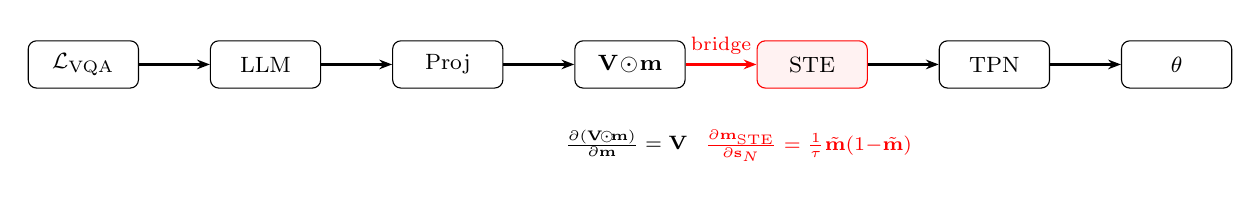
\begin{tikzpicture}[
    node distance=0.3cm and 0.9cm,
    block/.style={rectangle, draw, rounded corners=3pt,
                  minimum height=0.6cm, minimum width=1.4cm,
                  font=\footnotesize, align=center, fill=white},
    arr/.style={-{Stealth[scale=0.7]}, thick},
    rarr/.style={-{Stealth[scale=0.7]}, thick, red},
    eq/.style={font=\scriptsize, align=center},
]
  \node[block] (loss) {$\mathcal{L}_{\text{VQA}}$};
  \node[block, right=of loss] (llm) {LLM};
  \node[block, right=of llm] (proj) {Proj};
  \node[block, right=of proj] (mask) {$\mV\!\odot\!\vm$};
  \node[block, right=of mask, draw=red, fill=red!5] (ste) {STE};
  \node[block, right=of ste] (tpn) {TPN};
  \node[block, right=of tpn] (th) {$\theta$};

  \draw[arr] (loss) -- (llm);
  \draw[arr] (llm) -- (proj);
  \draw[arr] (proj) -- (mask);
  \draw[rarr] (mask) -- (ste) node[midway,above,eq,red]{bridge};
  \draw[arr] (ste) -- (tpn);
  \draw[arr] (tpn) -- (th);

  \node[below=0.4cm of mask, eq] {
    $\frac{\partial(\mV\!\odot\!\vm)}{\partial \vm} = \mV$
  };
  \node[below=0.4cm of ste, eq, red] {
    $\frac{\partial \vm_{\text{STE}}}{\partial \vs_N}
      = \frac{1}{\tau}\tilde{\vm}(1{-}\tilde{\vm})$
  };
\end{tikzpicture}
\caption{Gradient flow from VQA loss to TPN parameters. The STE (red) is
the critical differentiable bridge: without it, the discrete mask blocks
all gradients. Key partial derivatives shown below each node.}
\label{fig:grad_flow}
\end{figure}

The gradient at the masking point is:
\begin{equation}
  \frac{\partial (\mV \odot \vm)}{\partial \vm} = \mV
\end{equation}
The gradient w.r.t.\ the mask is the visual token itself (scaled by upstream
gradient). Via STE:
\begin{equation}
  \frac{\partial \vm_{\text{STE}}}{\partial \vs_N}
    = \frac{1}{\tau} \cdot \tilde{\vm} \odot (1 - \tilde{\vm})
\end{equation}

\paragraph{Why STE works despite bias.}
\begin{enumerate}[leftmargin=1.5em, itemsep=1pt]
  \item \textbf{Direction is correct}: if including token $i$ helps VQA,
    the STE gradient has the correct sign.
  \item \textbf{Low variance}: REINFORCE for 576 binary variables has
    variance $\sim\!2^{576}$. STE variance is $O(1)$ from Gumbel noise.
  \item \textbf{Annealing closes the gap}: as $\tau \to 0$, the soft mask
    converges to the hard mask, reducing bias.
\end{enumerate}

\subsection{Failure Mode Catalog}

\subsubsection{Failure Mode 1: Spatial Collapse (Center Bias)}

\begin{warnbox}[title={Spatial Collapse}]
\textbf{Symptom}: TPN selects center-image tokens regardless of query.
On a $24 \times 24$ heatmap, selections form a center blob.

\textbf{Cause}: Natural images have strong center bias (photographers center
subjects). TPN learns this prior instead of query-specific signals.

\textbf{Detection}: If mean selected-token centroid deviates from image
center $(11.5, 11.5)$ by less than $\epsilon = 2.0$ across validation set,
collapse has occurred.

\textbf{Fix}: Increase $|\mu|$ from 0.01 to 0.05. If persistent, add
explicit center-discounting bias to scores.
\end{warnbox}

\subsubsection{Failure Mode 2: Query Ignoring}

\begin{warnbox}[title={Query Ignoring}]
\textbf{Symptom}: For the same image, different queries produce nearly
identical token sets:
$\IoU(\mathcal{S}(\qe_1, \vc),\, \mathcal{S}(\qe_2, \vc)) \approx 1$.

\textbf{Cause}: $\mathbf{W}^Q$ collapses to near-zero; the TPN degenerates
to image-only selection.

\textbf{Detection}: Compute pairwise IoU across 100 query pairs on the same
images. If mean IoU $> 0.9$, query ignoring is occurring.

\textbf{Fix}: Extend Phase~0 (2 epochs), add $\mathcal{L}_{\text{div}}$,
monitor $\|\mathbf{W}^Q\|_F$ during training.
\end{warnbox}

\subsubsection{Failure Mode 3: Degenerate Fixed Mask}

\begin{warnbox}[title={Degenerate Fixed Mask}]
\textbf{Symptom}: Same $k$ tokens selected for every image and query.
Both spatial diversity and query sensitivity are zero.

\textbf{Cause}: Excessive $\lambda$ forces the TPN to find the single
``safest'' token set.

\textbf{Detection}: Pairwise IoU across all samples $> 0.95$.

\textbf{Fix}: Reduce $\lambda_{\max}$ by $10\times$, increase
$T_{\text{warmup}}$, reduce $\eta_{\text{LoRA}}$.
\end{warnbox}

\subsubsection{Failure Mode 4: Gradient Vanishing}

\begin{warnbox}[title={Gradient Vanishing Through STE}]
\textbf{Symptom}: TPN gradient norms drop by $>10\times$ within an epoch.

\textbf{Cause}: Temperature annealed too quickly; Gumbel-Sigmoid gradient
$\frac{1}{\tau}\tilde{m}(1{-}\tilde{m})$ becomes near-zero for most tokens.

\textbf{Detection}: Monitor \texttt{tpn\_grad\_norm} in wandb.

\textbf{Fix}: Use cosine annealing, or set $\tau_{\min} = 0.2$.
\end{warnbox}

\subsubsection{Failure Mode 5: LLM Bypassing Visual Channel}

\begin{warnbox}[title={LLM Language-Prior Bypass}]
\textbf{Symptom}: VQA accuracy unchanged when mask is randomly permuted.

\textbf{Cause}: LoRA adapts too quickly; LLM answers from language priors
alone, making visual tokens irrelevant.

\textbf{Fix}: Reduce $\eta_{\text{LoRA}}$, extend Phase~0.
\end{warnbox}

% ════════════════════════════════════════════════════════════════════════════
\section{Experimental Design}
\label{sec:experiments}
% ════════════════════════════════════════════════════════════════════════════

\subsection{Setup}

\paragraph{Backbone.}
LLaVA-1.5-7B (CLIP ViT-L/14, Vicuna-7B).
Default: $k = 144$ ($4\times$ compression).

\paragraph{Datasets.}
\begin{itemize}[leftmargin=1.5em, itemsep=1pt]
  \item \textbf{VQAv2}: 214K images, 1.1M QA pairs. Primary benchmark.
  \item \textbf{GQA}: $\sim$1M balanced QA pairs with spatial-relation
    annotations.
  \item \textbf{TextVQA}: OCR-dependent VQA.
  \item \textbf{POPE}: adversarial binary questions for hallucination.
\end{itemize}

\paragraph{Metrics.}
VQA-Score (official accuracy), GQA exact-match, POPE F1, end-to-end
latency at batch size 1 on A100.

\subsection{Baselines}

\begin{table}[h]
\centering
\caption{Baseline conditions (all use LLaVA-1.5-7B, $k{=}144$ except
full model).}
\label{tab:baselines}
\renewcommand{\arraystretch}{1.15}
\small
\begin{tabular}{@{}lccp{5cm}@{}}
  \toprule
  Condition & Query-Aware & Tokens & Description \\
  \midrule
  LLaVA-1.5 (full) & N/A & 576 & Upper bound \\
  Random drop & No & 144 & Uniformly random subset \\
  ToMe & No & 144 & Bipartite soft matching \\
  Image-only TPN (A3) & No & 144 & TPN with $\qe$ zeroed \\
  \textbf{TC-ViTok} & \textbf{Yes} & \textbf{144} & \textbf{Full method} \\
  \bottomrule
\end{tabular}
\end{table}

\subsection{Spatial Specificity Protocol}

Questions are classified as \emph{spatial} or \emph{global} by priority:
\begin{enumerate}[leftmargin=1.5em, itemsep=1pt]
  \item (GQA only) Semantic annotation: \texttt{relation.spatial = True}.
  \item Answer is spatial direction (``left,'' ``right,'' etc.).
  \item Question contains spatial keywords from a predefined set.
\end{enumerate}

\subsection{Ablation Matrix}

\begin{table}[h]
\centering
\caption{Complete ablation matrix.}
\label{tab:ablations}
\renewcommand{\arraystretch}{1.15}
\small
\begin{tabular}{@{}llp{5.5cm}@{}}
  \toprule
  ID & Variation & What It Tests \\
  \midrule
  A1 & Full TC-ViTok & Full system performance \\
  A2 & Random drop & Absolute lower bound \\
  A3 & Image-only TPN & Value of query-conditioning \\
  A4 & $k \in \{72,144,216,288\}$ & Pareto frontier \\
  A5 & Spatial vs.\ global split & Core hypothesis \\
  \midrule
  B1 & Skip Phase~0 & Cold-start importance \\
  B2 & Fixed $\tau{=}1.0$ & Annealing importance \\
  B3 & DINOv2-S vs.\ CLIP-B coarse & Encoder suitability \\
  \bottomrule
\end{tabular}
\end{table}

\subsection{Hypotheses}

\begin{hypothesis}[Query-Conditioning Selectivity]
  \label{hyp:main}
  For spatially-grounded VQA questions, TC-ViTok (A1) achieves strictly
  higher accuracy than image-only TPN (A3) at the same $k$. For
  globally-answerable questions, A1 and A3 perform comparably:
  \begin{align}
    \text{Acc}(\text{A1},\,\text{spatial})
      &> \text{Acc}(\text{A3},\,\text{spatial}) \\
    |\text{Acc}(\text{A1},\,\text{global})
      - \text{Acc}(\text{A3},\,\text{global})|
      &\approx 0
  \end{align}
\end{hypothesis}

\begin{hypothesis}[Pareto Dominance]
  \label{hyp:pareto}
  The accuracy-vs-tokens Pareto curve of TC-ViTok lies at or above all
  query-agnostic baselines for $k \in \{72, 144, 216, 288\}$.
\end{hypothesis}

\subsection{Projected Results}

\begin{table}[h]
\centering
\caption{\textbf{Projected} results (not yet measured). All numbers will
be replaced by measured results.}
\label{tab:projected}
\renewcommand{\arraystretch}{1.2}
\small
\begin{tabular}{@{}lccccr@{}}
  \toprule
  Method & VQAv2 & GQA & GQA-spat. & POPE-F1 & Tokens \\
  \midrule
  LLaVA-1.5 (full) & 79.1 & 63.3 & 62.1 & 85.9 & 576 \\
  Random drop & $\sim$72 & $\sim$57 & $\sim$53 & $\sim$81 & 144 \\
  ToMe & $\sim$74 & $\sim$59 & $\sim$55 & $\sim$83 & 144 \\
  Image-only TPN & $\sim$75 & $\sim$60 & $\sim$56 & $\sim$83 & 144 \\
  \textbf{TC-ViTok} & $\mathbf{\sim\!76}$ & $\mathbf{\sim\!61}$
    & $\mathbf{\sim\!59}$ & $\mathbf{\sim\!84}$ & \textbf{144} \\
  \bottomrule
\end{tabular}
\end{table}

\paragraph{Interpreting weaker-than-expected results.}
If overall VQA improvement is $< 0.5$ points, the work remains informative
provided: (i)~spatial/global split confirms predicted asymmetry;
(ii)~Pareto curve shows advantage grows with compression ratio;
(iii)~qualitative masks show semantic patterns. If A1 does not outperform
A3 at all, this is a clean negative result: CLIP [EOS] does not provide
sufficient spatial guidance.

% ════════════════════════════════════════════════════════════════════════════
\section{Empirical Validation and Analysis}
\label{sec:validation}
% ════════════════════════════════════════════════════════════════════════════

\subsection{Evaluation Pipeline}

\begin{lstlisting}[caption={Evaluation with spatial stratification.}]
@torch.no_grad()
def evaluate(model, val_dataset, k, device='cuda'):
    model.eval()
    correct = {'overall': 0, 'spatial': 0, 'global': 0}
    total   = {'overall': 0, 'spatial': 0, 'global': 0}

    for batch in tqdm(DataLoader(val_dataset, batch_size=1)):
        pred, mask = inference(model, batch, k)
        is_correct = vqa_accuracy(pred, batch['answer'])

        cat = 'spatial' if classify_spatial(
            batch['question'], batch['answer']) else 'global'
        correct['overall'] += is_correct
        correct[cat] += is_correct
        total['overall'] += 1
        total[cat] += 1

    return {key: correct[key]/max(total[key],1)*100
            for key in correct}
\end{lstlisting}

\subsection{Latency Measurement}

\begin{lstlisting}[caption={GPU-accurate latency measurement.}]
def measure_latency(model, dataset, k_values, n_measure=100):
    results = {}
    for k in k_values:
        # Warmup
        for i in range(10):
            _ = inference(model, dataset[i], k)
        torch.cuda.synchronize()

        start = torch.cuda.Event(enable_timing=True)
        end   = torch.cuda.Event(enable_timing=True)
        times = []

        for i in range(n_measure):
            torch.cuda.synchronize()
            start.record()
            _ = inference(model, dataset[i], k)
            end.record()
            torch.cuda.synchronize()
            times.append(start.elapsed_time(end))

        results[k] = {'mean': np.mean(times),
                       'std': np.std(times)}
    return results
\end{lstlisting}

\subsection{Mask Visualization}

\begin{lstlisting}[caption={Token selection overlay visualization.}]
def visualize_mask(image, mask, question, k=144):
    import matplotlib.pyplot as plt
    fig, axes = plt.subplots(1, 3, figsize=(15, 5))

    axes[0].imshow(image)
    axes[0].set_title("Original")

    mask_2d = mask.reshape(24, 24).cpu().numpy()
    axes[1].imshow(mask_2d, cmap='hot', interpolation='nearest')
    axes[1].set_title(f"Selected (k={k})")

    axes[2].imshow(image, alpha=0.5)
    overlay = F.interpolate(
        torch.tensor(mask_2d).float()[None, None],
        size=image.shape[:2], mode='nearest'
    ).squeeze().numpy()
    axes[2].imshow(overlay, cmap='Greens', alpha=0.4)
    axes[2].set_title(f"Q: {question[:50]}...")
    plt.tight_layout()
    plt.savefig('mask_viz.pdf', dpi=150)
\end{lstlisting}

\subsection{What Results Validate vs.\ Invalidate the Idea}

\begin{keybox}[title={Validation Criteria}]
\textbf{Validated if:}
\begin{enumerate}[leftmargin=1.5em, itemsep=1pt]
  \item $\text{Acc}(\text{A1}, \text{spatial}) >
    \text{Acc}(\text{A3}, \text{spatial})$ with $p < 0.05$
  \item $|\text{Acc}(\text{A1}, \text{global}) -
    \text{Acc}(\text{A3}, \text{global})| < 0.5\%$
  \item Mask visualizations show query-specific spatial patterns
  \item Pareto curve: TC-ViTok at or above all baselines
\end{enumerate}

\textbf{Partially validated if:}
Overall gain $< 0.5\%$ but spatial-specific gain $> 1\%$ with clear
asymmetry.

\textbf{Invalidated if:}
A1 $\approx$ A3 on both spatial and global questions, and masks show no
query sensitivity ($\text{IoU} \approx 1$ across query pairs).
\end{enumerate}
\end{keybox}

% ════════════════════════════════════════════════════════════════════════════
\section{Interpretation and Insights}
\label{sec:interpretation}
% ════════════════════════════════════════════════════════════════════════════

\subsection{When TC-ViTok Works Best}

\begin{itemize}[leftmargin=1.5em, itemsep=2pt]
  \item \textbf{Spatially localized questions}: ``What color is the shirt
    of the person on the left?''
  \item \textbf{OCR/text reading}: ``What does the sign say?'' --- TPN
    focuses on text regions.
  \item \textbf{Counting in specific regions}: ``How many people are
    sitting?''
  \item \textbf{Spatial relation questions}: ``Is the cat to the left or
    right of the dog?''
\end{itemize}

\subsection{When TC-ViTok May Not Help}

\begin{itemize}[leftmargin=1.5em, itemsep=2pt]
  \item \textbf{Global scene understanding}: ``Is this indoors or
    outdoors?'' --- any token subset suffices.
  \item \textbf{Simple yes/no}: ``Is there a car?'' --- LLM answers from
    language priors.
  \item \textbf{Dominant-object questions}: center bias already captures
    these.
\end{itemize}

\subsection{Diagnostic Monitoring}

\begin{table}[h]
\centering
\caption{Key metrics to monitor during training.}
\label{tab:diagnostics}
\renewcommand{\arraystretch}{1.2}
\small
\begin{tabular}{@{}llll@{}}
  \toprule
  Metric & Healthy & Warning & Action \\
  \midrule
  Mean centroid & Varies by query & Always $(12,12)$
    & Increase $|\mu|$ \\
  Cross-query IoU & $< 0.7$ & $> 0.9$
    & Extend Phase~0, add $\mathcal{L}_{\text{div}}$ \\
  TPN grad norm & $> 0.01$ & $< 0.001$
    & Slow $\tau$ annealing \\
  $\|\mathbf{W}^Q\|_F$ & $> 1.0$ & $< 0.1$
    & Query pathway collapsing \\
  VQA loss (Phase~0) & Decreasing & Flat
    & TPN not learning \\
  Score L1 norm & Decreasing & Increasing
    & $\lambda$ too weak \\
  \bottomrule
\end{tabular}
\end{table}

% ════════════════════════════════════════════════════════════════════════════
\section{Execution Roadmap}
\label{sec:roadmap}
% ════════════════════════════════════════════════════════════════════════════

\begin{table}[h]
\centering
\caption{Week-by-week execution plan.}
\label{tab:roadmap}
\renewcommand{\arraystretch}{1.25}
\small
\begin{tabular}{@{}clp{6.5cm}l@{}}
  \toprule
  Week & Phase & Key Tasks & Milestone \\
  \midrule
  1 & Setup &
    Install dependencies, download models, run LLaVA baseline,
    implement feature caching &
    Baseline accuracy confirmed \\
  2 & Build &
    Implement Gumbel-STE, TPN module, debug checks,
    TCViTok wrapper &
    Full fwd/bwd pass works \\
  3 & Train I &
    Implement loss functions, Phase~0 loop,
    Phase~1 with schedules, wandb logging &
    First trained model \\
  4 & Train II &
    Full training protocol, failure mode detection,
    fix issues, retrain if needed &
    Clean model passes checks \\
  5 & Experiments &
    Train A3 ablation, run all baselines at $k{=}144$,
    $k$-sweep, spatial analysis &
    Main results table \\
  6 & Analysis &
    Mask visualizations, latency measurements,
    remaining ablations, write paper &
    Complete draft \\
  \bottomrule
\end{tabular}
\end{table}

% ════════════════════════════════════════════════════════════════════════════
\section{Quick Reference}
\label{sec:reference}
% ════════════════════════════════════════════════════════════════════════════

\begin{keybox}[title={Key Numbers at a Glance}]
\renewcommand{\arraystretch}{1.15}
\small
\begin{tabular}{@{}lr||lr@{}}
  Full visual tokens $N$ & 576 &
    TPN parameters & $\sim$0.9\,M \\
  Token budget $k$ & 144 (default) &
    LoRA parameters & $\sim$25\,M \\
  Compression ratio & $4\times$ &
    DINOv2-S latency & $\sim$3\,ms \\
  Coarse tokens $M$ & 49 &
    CLIP text latency & $\sim$2\,ms \\
  $d_{\text{model}}$ & 384 &
    TPN latency & $\sim$0.5\,ms \\
  Heads $H$ & 4 &
    Total overhead & $\sim$5.5\,ms \\
  $\tau_{\max} \to \tau_{\min}$ & $1.0 \to 0.1$ &
    LLM savings & $\sim$40\,ms \\
  $\lambda_{\max}$ & 0.1 &
    Net savings & $\sim$34\,ms \\
  $|\mu|$ & 0.01 &
    Phase~0 & 1 epoch (TPN only) \\
  $\gamma$ (diversity margin) & 0.5 &
    Phase~1 & 3 epochs (joint) \\
\end{tabular}
\end{keybox}

% ════════════════════════════════════════════════════════════════════════════
% References
% ════════════════════════════════════════════════════════════════════════════

\begin{thebibliography}{99}

\bibitem{bai2023qwenvl}
Bai, J., et al.\ (2023).
Qwen-VL: A versatile vision-language model.
\emph{arXiv:2308.12966}.

\bibitem{bengio2013estimating}
Bengio, Y., L\'{e}onard, N., \& Courville, A.\ (2013).
Estimating or propagating gradients through stochastic neurons.
\emph{arXiv:1308.3432}.

\bibitem{bolya2022token}
Bolya, D., et al.\ (2023).
Token merging: Your ViT but faster.
In \emph{ICLR}.

\bibitem{goyal2017vqa}
Goyal, Y., et al.\ (2017).
Making the V in VQA matter.
In \emph{CVPR}.

\bibitem{hu2022lora}
Hu, E.~J., et al.\ (2022).
LoRA: Low-rank adaptation of large language models.
In \emph{ICLR}.

\bibitem{hudson2019gqa}
Hudson, D.~A., \& Manning, C.~D.\ (2019).
GQA: A new dataset for real-world visual reasoning.
In \emph{CVPR}.

\bibitem{jang2017categorical}
Jang, E., Gu, S., \& Poole, B.\ (2017).
Categorical reparameterization with Gumbel-Softmax.
In \emph{ICLR}.

\bibitem{li2023blip2}
Li, J., et al.\ (2023).
BLIP-2: Bootstrapping language-image pre-training.
In \emph{ICML}.

\bibitem{liang2022evit}
Liang, Y., et al.\ (2022).
Not all patches are what you need.
In \emph{ICLR}.

\bibitem{liu2024llava}
Liu, H., et al.\ (2023).
Visual instruction tuning.
In \emph{NeurIPS}.

\bibitem{maddison2017concrete}
Maddison, C.~J., Mnih, A., \& Teh, Y.~W.\ (2017).
The Concrete distribution.
In \emph{ICLR}.

\bibitem{meng2022adavit}
Meng, L., et al.\ (2022).
AdaViT: Adaptive vision transformers.
In \emph{CVPR}.

\bibitem{oquab2023dinov2}
Oquab, M., et al.\ (2023).
DINOv2: Learning robust visual features without supervision.
\emph{arXiv:2304.07193}.

\bibitem{pope}
Li, Y., et al.\ (2023).
Evaluating object hallucination in large vision-language models.
In \emph{EMNLP}.

\bibitem{radford2021learning}
Radford, A., et al.\ (2021).
Learning transferable visual models from natural language supervision.
In \emph{ICML}.

\bibitem{rao2021dynamicvit}
Rao, Y., et al.\ (2021).
DynamicViT: Efficient vision transformers with dynamic token
sparsification.
In \emph{NeurIPS}.

\bibitem{shang2024llava}
Shang, Y., et al.\ (2024).
LLaVA-PruMerge: Adaptive token reduction.
\emph{arXiv:2403.15388}.

\bibitem{shazeer2017moe}
Shazeer, N., et al.\ (2017).
Outrageously large neural networks: The sparsely-gated
mixture-of-experts layer.
In \emph{ICLR}.

\bibitem{teerapittayanon2016branchynet}
Teerapittayanon, S., et al.\ (2016).
BranchyNet: Fast inference via early exiting.
In \emph{ICPR}.

\end{thebibliography}

\end{document}